\documentclass[sigconf,review]{acmart}
\usepackage{enumitem}
\usepackage{booktabs}
\usepackage{multirow}
\usepackage{placeins}
\usepackage[most]{tcolorbox}
\settopmatter{printacmref=false, printccs=true, printfolios=true}
\setcopyright{none}
\acmConference[CIKM '26]{The 35th ACM International Conference on Information and Knowledge Management}{November 9--11, 2026}{Rome, Italy}
\acmISBN{}
\acmDOI{}
\acmYear{2026}
\copyrightyear{2026}

\begin{document}

\title{TelecomAudit: Origin-Aware Benchmark Auditing and Calibration for 5G Anomaly Detection
% When Synthetic Telecom Benchmarks Miss Controlled-Real 5G Faults: Origin-Aware Auditing and Calibration
% title 2 recommendation: Origin-Aware Auditing for Synthetic Telecom Anomaly Benchmarks
% title 3 recommendation: Auditing Synthetic Telecom Benchmarks for Controlled-Real 5G Fault Coverage
}

\author{Chiman Salavati}
% \authornote{Corresponding author.}
\affiliation{%
  \institution{University of Connecticut}
  \city{Storrs}
  \state{CT}
  \country{USA}}
\email{chiman.salavati@uconn.edu}

\author{Liang Wu}
\affiliation{%
  \institution{Nokia}
  \city{Sunnyvale}
  \state{California}
  \country{USA}}
\email{liang.wu@nokia.com}

\author{Kelly Wan}
\affiliation{%
  \institution{Nokia}
  \city{Sunnyvale}
  \state{California}
  \country{USA}}
\email{kelly.wan@nokia.com}

\author{Mayank Darbari}
\affiliation{%
  \institution{Nokia}
  \city{Sunnyvale}
  \state{California}
  \country{USA}}
\email{mayank.darbari@nokia.com}

\author{Liangjie Hong}
\affiliation{%
  \institution{Nokia}
  \city{Sunnyvale}
  \state{California}
  \country{USA}}
\email{liangjie.hong@nokia.com}

\renewcommand{\shortauthors}{Salavati et al.}

\begin{abstract}
Modern wireless networks increasingly support reliability-critical applications, from industrial automation and autonomous mobility to UAV connectivity, making anomaly detection critical for dependable 5G and self-optimizing 6G operations. Yet labeled telecom faults are rare, costly to annotate, and difficult to release, so many telecom anomaly detectors are trained and evaluated using injected, generated, or simulated anomalies. This raises an important deployment question: can strong synthetic-benchmark performance be trusted for operational detector selection? Rather than assuming synthetic anomalies are valid proxies for deployment-relevant faults, we ask whether benchmark anomalies cover the KPI regimes occupied by controlled-real faults, and we operationalize this question as \emph{origin-aware benchmark auditing}: a deployment-oriented evaluation workflow that explicitly conditions evaluation on anomaly origin. Across two public 5G/Open RAN testbed corpora, the audit exposes an operational failure hidden by aggregate metrics: synthetic-only training can retain strong performance on synthetic anomalies while missing controlled-real fault regimes under deployment-relevant operating conditions. We provide evidence that this failure reflects an operating-regime coverage gap rather than a model-specific limitation or feature leakage, and that modest controlled-real calibration substantially improves controlled-real detection where additional synthetic or normal data, and synthetic reweighting do not. We release a reproducible audit toolkit and artifacts, and an operator checklist for deployment-oriented benchmark validation, together with industrial validation as a pre-production shadow-mode CI gate within Nokia's anomaly-detection pipeline.
\end{abstract}

\begin{CCSXML}
<ccs2012>
 <concept>
  <concept_id>10010147.10010257</concept_id>
  <concept_desc>Computing methodologies~Machine learning</concept_desc>
  <concept_significance>500</concept_significance>
 </concept>
 <concept>
  <concept_id>10002951.10003317</concept_id>
  <concept_desc>Information systems~Data mining</concept_desc>
  <concept_significance>300</concept_significance>
 </concept>
</ccs2012>
\end{CCSXML}
\ccsdesc[500]{Computing methodologies~Machine learning}
\ccsdesc[300]{Information systems~Data mining}

\keywords{5G anomaly detection, benchmark auditing, distribution shift, synthetic-to-real transfer, telecom observability, Open RAN}

\maketitle
%% ====================================================================
\section{Introduction}
\label{sec:intro}

Reliable anomaly detection is a core requirement for 5G operations and an increasingly important prerequisite for autonomous 6G networks. Modern Radio Access Network (RAN) deployments generate high-dimensional streams of Key Performance Indicators (KPIs), such as signal quality, throughput, and resource-utilization metrics, that can reveal radio interference, congestion, software faults, mobility failures, and scheduling problems. However, these signals are useful only if detectors trained offline transfer to the operating conditions encountered during deployment. Real telecom failures are rare, operator datasets are difficult to release, and expert labeling is expensive, so many telecom anomaly studies evaluate detectors using injected, generated, or simulated anomalies~\citep{wu2018cellpad,wang2021tsagen,hasan2024simba}. These choices are practical, but they leave an important benchmark assumption largely untested: whether synthetic anomalies adequately cover the operating regimes occupied by real Radio-Frequency (RF) faults observed in controlled 5G/Open RAN testbeds.

To study when synthetic telecom anomalies fail to transfer to deployment-relevant operating conditions, we evaluate two independent public 5G/Open RAN testbed datasets: TelecomTS~\citep{feng2025telecomts} and SpotLight~\citep{sun2024spotlight}. TelecomTS contains both real radio-frequency interference events collected in a controlled testbed environment and ten synthetic anomaly types generated through KPI perturbations. SpotLight similarly combines controlled radio-interference events with several synthetic protocol- and network-level anomaly types. Importantly, the dominant signals separating real and synthetic anomalies differ across the two datasets: TelecomTS is driven primarily by signal-strength behavior (RSRP), while SpotLight is separated mainly by layer-2 radio-control statistics. 

Throughout this paper, we use \emph{controlled-real} to describe anomalies injected through physical RF or hardware mechanisms and observed through a real network stack, rather than passively collected outages from operational cellular deployments. Some observed mismatches arise from dataset collection procedures themselves, such as differences in device placement during fault collection, rather than from the synthetic-anomaly generators alone. The audit is designed to expose either source of mismatch during benchmark validation. Across both datasets, the audit reveals two linked effects: a \emph{distributional gap}, in which controlled-real and synthetic anomalies occupy different KPI operating regimes, and a \emph{transfer gap}, in which detectors trained only on synthetic anomalies continue to detect synthetic faults while failing on controlled-real ones. As a result, aggregate benchmark metrics can remain high even when deployment-relevant faults are missed.

This work treats anomaly origin as an explicit benchmark variable during deployment-oriented anomaly detection evaluation, and operationalizes this perspective as an applied audit workflow with a released toolkit and pre-production integration into Nokia's in-house anomaly-detection platform.
Our main contributions are:

\begin{itemize}[leftmargin=*,nosep]
  \item We operationalize \emph{origin-aware benchmark auditing}, a deployment-oriented evaluation workflow that explicitly accounts for anomaly origin during telecom benchmark validation.

  \item We show that synthetic-only training can retain strong performance on synthetic anomalies while failing on controlled-real fault regimes across multiple detector families and evaluation settings, and that this failure replicates on the independent SpotLight Open RAN corpus.

  \item We provide evidence that the failure reflects an operating-regime coverage gap rather than a simple feature-leakage artifact or recorded deployment-context mismatch.

  \item We show that modest controlled-real calibration substantially improves controlled-real detection, whereas additional synthetic data, additional normal data, and synthetic reweighting do not recover controlled-real recall in the same way.

  \item We validate \emph{TelecomAudit} across two independent public 5G/Open RAN testbeds, release a reproducible audit toolkit and operator checklist, and integrate the audit as a pre-production shadow-mode CI gate inside Nokia's anomaly-detection platform.
\end{itemize}
%% ====================================================================
\section{Related Work}
\label{sec:related}

\subsection{Telecom benchmarks and synthetic anomalies}
TelecomTS provides absolute-scale 5G KPI traces with both controlled Jamming and synthetic anomaly types~\citep{feng2025telecomts}, while SpotLight studies explainable anomaly detection on an Open RAN testbed with mixed Radio/Pdcp/Mac/Network anomalies~\citep{sun2024spotlight}. CellPAD~\citep{wu2018cellpad} evaluates KPI anomaly detection using injected LTE anomalies, while TSAGen~\citep{wang2021tsagen} and Simba~\citep{hasan2024simba} rely on generated or simulator-injected cellular anomalies. BOOM/Toto broadens observability benchmarking to large-scale production metrics~\citep{cohen2025toto}. These works motivate controlled and synthetic anomaly generation, whereas we study when such anomalies fail to transfer to controlled-real fault regimes and operationalize this analysis as a reproducible audit.

\subsection{Anomaly detection and protocol auditing}
A large body of work develops KPI and multivariate anomaly detectors for operational systems~\citep{liu2015opprentice,xu2018donut,ren2019microsoft,yu2023autokad,su2019omnianomaly,audibert2020usad}, and recent time-series foundation models have become common baselines for downstream tasks~\citep{goswami2024moment,cohen2025toto,feofanov2025mantis,ansari2024chronos}. A complementary line of work audits evaluation protocols: point-adjustment can inflate TSAD scores~\citep{kim2022pointadjust}, simple baselines can match deep detectors~\citep{audibert2022usadrevisited}, one-liner baselines can match foundation-model anomaly scores under fixed protocols~\citep{zhu2026oneliners}, and benchmarking efforts such as TimeEval/TSB-AD push reproducible evaluation~\citep{wenig2022timeeval,liu2024tsbad}. These audits generally assume a fixed anomaly-label space. In contrast, we audit whether anomalies from different origins constitute valid proxies for the controlled-real fault population. Our setting is therefore complementary to metric-reliability auditing.

\subsection{Distribution shift, domain adaptation, and subgroup failure}
Under the standard dataset-shift taxonomy~\citep{quinonero2009shift,morenotorres2012unifying}, the real--synthetic gap corresponds to origin-conditional covariate shift: controlled-real and synthetic anomaly windows exhibit different $P(X\!\mid\!\textsc{origin})$ despite sharing the same anomaly label, so detectors trained on an aggregate anomaly distribution can fail when controlled-real faults occupy different KPI operating regimes. We use classifier two-sample tests~\citep{lopezpaz2017c2st} and kernel MMD~\citep{gretton2012mmd} as diagnostic tools rather than as new detection methods, and compare against importance-weighted training and uLSIF-style covariate-shift correction~\citep{sugiyama2007covariate,kanamori2009ulsif,bickel2009dasvm}. Related perspectives also appear in work on shortcut learning~\citep{geirhos2020shortcut}, hidden stratification in clinical ML~\citep{oakden2020hidden}, dataset-audit or benchmark-artifact studies~\citep{recht2019imagenet}, and on field non-stationarity in deployed AIOps alert streams~\citep{bhukar2024dynamic}. TelecomAudit framework operationalizes subgroup-failure analysis for telecom anomaly benchmarking by treating anomaly origin as an explicit deployment variable during benchmark validation and model-promotion decisions.
%% ====================================================================

\section{Benchmark and Audit Protocol}
\label{sec:setup}

\subsection{Anomaly-origin definition}
In this study, \textbf{controlled-real} refers to anomalies injected through RF or hardware mechanisms and observed through a real RAN stack in a testbed environment (TelecomTS Jamming; SpotLight \textsc{Radio}). \textbf{Synthetic} refers to benchmark anomaly types generated without physical RF or hardware fault injection, including the ten non-Jamming TelecomTS types and SpotLight \textsc{Pdcp}/\textsc{Mac}/\textsc{Network}. \textbf{Field-real} refers to passively observed outages collected from deployed operational networks. Neither corpus contains field-real anomalies; our claims therefore concern transfer from synthetic benchmark anomalies to controlled-real testbed faults, not generalization to passively observed operational outages.
\subsection{Origin-aware audit}
Let $x_i\in\mathbb{R}^{T\times d}$ denote a KPI window, $y_i\in\{0,1\}$ its anomaly label, and $o_i\in\{\textsc{synthetic},\textsc{controlled}\}$ the anomaly origin. A detector produces an anomaly score $s_\theta(x)$ and prediction
\[
\hat y_{\theta,\tau}(x)=\mathbf{1}\{s_\theta(x)\ge\tau\},
\]
where $\tau$ is a decision threshold selected on validation data and fixed for testing. In addition to aggregate $F_1$ and AUROC, the audit reports origin-conditioned recall
\[
\widehat R_o=
\frac{\sum_i \mathbf{1}\{y_i=1,\,o_i=o,\,\hat y_{\theta,\tau}(x_i)=1\}}
{\sum_i \mathbf{1}\{y_i=1,\,o_i=o\}},
\quad
o\in\{\textsc{s},\textsc{c}\}.
\]
where $s$ denotes synthetic anomalies and $c$ denotes controlled-real anomalies.
We define the empirical transfer gap as
\[
\widehat G_{\mathrm{tr}}
=
\widehat R_{\textsc{s}}
-
\widehat R_{\textsc{c}},
\]
so large positive values indicate detectors that recognize synthetic anomalies while missing controlled-real faults. Distributional coverage is evaluated by comparing
\[
P(\phi(X)\mid O=\textsc{s},Y=1)
\quad \text{vs.} \quad
P(\phi(X)\mid O=\textsc{c},Y=1),
\]
using classifier two-sample tests (C2ST)~\citep{lopezpaz2017c2st} and kernel maximum mean discrepancy (MMD) diagnostics~\citep{gretton2012mmd}.

\subsection{Corpora}
TelecomTS~\citep{feng2025telecomts} contains 32{,}000 windows (30{,}765 normal, 1{,}235 anomalous; 11 anomaly types) of 128 timesteps over 16 numeric KPI channels covering radio/PHY (RSRP, UL\_SNR\footnote{\textbf{KPI primer.} RSRP = Reference Signal Received Power (downlink signal-quality indicator, dBm). UL\_SNR = Uplink Signal-to-Noise Ratio. DL/UL\_BLER = Block Error Rate per direction. DL/UL\_MCS = Modulation \& Coding Scheme index. PRB = Physical Resource Block (RAN scheduler unit). RLC (used on SpotLight, \S\ref{sec:cross-corpus}) = Radio Link Control, layer-2 protocol counters.}), error rates (DL/UL\_BLER), modulation/coding (DL/UL\_MCS), scheduler/resource (PRB utilisation, current PRBs, UL\_NPRB, estimated UL buffer), and traffic counters (TX/RX bytes and packet counts). SpotLight~\citep{sun2024spotlight} is a public Open RAN dataset from an independent 5G testbed with 241 controlled-real \textsc{Radio} windows and 436 synthetic windows of 64 timesteps over 452 RAN/platform channels. TelecomTS metadata also includes deployment context (zone, application, mobility, congestion). We use this metadata only for context and split-sensitivity audits; detector inputs remain restricted to numeric KPI channels. 

\subsection{Features and primary diagnostic detector}
For tabular diagnostics, we map each KPI window $x$ to a summary vector $\phi(x)\in\mathbb{R}^{240}$ using 15 statistics per KPI: level, dispersion, trend, change-energy, autocorrelation, and spectral descriptors. This representation is used for per-KPI tests, C2ST~\citep{lopezpaz2017c2st}, MMD~\citep{gretton2012mmd}, train-on-synthetic/test-on-real (TSTR) detection, calibration, and single-KPI sanity checks. The primary diagnostic detector is \texttt{HistGradientBoostingClassifier}~\citep{pedregosa2011sklearn}; the goal is benchmark auditing rather than proposing a new detector architecture. We assess model-family robustness by repeating the TSTR protocol with additional tabular detectors including XGBoost~\citep{chen2016xgboost} and raw-window detectors (which consume the full $128\times16$ KPI tensor with no engineered summary) in \S\ref{sec:real-synth}.

\subsection{Splits and evaluation}
We use task-specific partitions (Table~\ref{tab:splits}). The \emph{full-scale} split preserves the natural 3.9\% anomaly rate and is used for the main deployment-oriented TSTR and calibration experiments, with all controlled-real Jamming windows excluded from synthetic-only training. The remaining splits support diagnostic analysis: the \emph{controlled-500} split isolates origin transfer by balancing controlled-real and synthetic counts in the test set; the \emph{balanced-detection} split supports single-KPI sensitivity analysis at a 50\% anomaly rate; and the \emph{context LOO} partitions hold out one deployment-context value at a time.

The training partition is further divided into train and validation
subsets. Decision thresholds are tuned only on the validation subset
(by maximizing $F_1$) and are frozen before any evaluation on the
held-out test set. To prevent threshold selection from obscuring
origin-specific failures, we report origin-conditioned recalls and
AUROC alongside aggregate $F_1$.

The released windows are fixed and non-overlapping, so we shuffle
windows within each partition using a fixed random seed. This avoids
adjacent-window overlap leakage, although residual dependence
between windows originating from the same underlying trace or
session may still remain. Base train/validation/test partitions are
fixed once, while stochastic model initialization and calibration
subsampling are repeated over ten additional random seeds. The controlled-real test pool remains fully disjoint from
the calibration pool for every sweep value $f$ and every random
seed. Per-trace or per-session group-aware splits would provide a
stricter estimate of generalization, but released TelecomTS metadata
does not include session identifiers; we return to this limitation in
\S\ref{sec:conclusion-limits}.

\begin{table}[t]
  \caption{TelecomTS audit partitions.}
  \label{tab:splits}
  \small
  \setlength{\tabcolsep}{2.5pt}
  \begin{tabular}{@{}llcc@{}}
    \toprule
    \textbf{Partition} & \textbf{Primary use} & \textbf{Train/Val/Test} & \textbf{Anom.\ rate} \\
    \midrule
    Full-scale     & TSTR and calibration  & 25{,}600/--/6{,}400 & 3.9\% \\
    Balanced det.  & KPI sensitivity       & 1580/396/494 & 50\% \\
    Controlled-500 & Origin transfer       & 300/100/100 & 50\% \\
    Context LOO    & Context sensitivity   & all other/--/held-out & variable \\
    \bottomrule
  \end{tabular}
\end{table}

%% ====================================================================
\section{Diagnosing and Repairing the Real--Synthetic Gap}
\label{sec:analysis}
%% ====================================================================

Our audit framework evaluates two linked effects: a distributional gap between controlled-real and synthetic anomaly windows in KPI-summary space, and a transfer gap in which models trained only on synthetic anomalies fail to detect controlled-real faults. Aggregate binary $F_1$ can remain high even when the controlled-real origin is missed entirely.

\subsection{Synthetic-Only Training Fails Across Detector Families}
\label{sec:real-synth}

Table~\ref{tab:e9_transfer} evaluates whether detectors trained on synthetic anomalies transfer to controlled-real faults across four evaluation regimes. \emph{Ctrl-500 / all} trains on both synthetic and controlled-real anomalies and tests on a balanced controlled-real/synthetic split, while \emph{Ctrl-500 / synth} uses the same test split but removes all controlled-real Jamming windows from training. \emph{Bal-494 / synth} and \emph{Full-6.4k / synth} evaluate synthetic-only training on the larger balanced-detection and deployment-oriented full-scale splits, respectively.

The table spans multiple detector families: six tabular models trained on engineered KPI summaries together with five supervised raw-window detectors operating on $128\times16$ KPI windows, including frozen foundation-model encoders (Toto~\citep{cohen2025toto}, Mantis~\citep{feofanov2025mantis}) and end-to-end deep classifiers (TimesNet~\citep{wu2023timesnet}, InceptionTime~\citep{ismail2020inceptiontime}, PatchTST~\citep{nie2023patchtst}). All values are mean $\pm$ standard deviation over ten random seeds.

The \emph{Ctrl-500} regimes isolate the effect of training composition. When both synthetic and controlled-real anomalies appear during training (\emph{Ctrl-500 / all}), detectors recover both origins across nearly all architectures. Once controlled-real Jamming is removed from training (\emph{Ctrl-500 / synth}), controlled-real recall collapses while synthetic-anomaly recall remains high, showing that the transfer failure is detector-family independent.

The most deployment-relevant evidence comes from the \emph{Full-6.4k / synth} regime at the natural 3.9\% anomaly rate. Under synthetic-only training, nearly every detector misses controlled-real Jamming while aggregate $F_1$ and AUROC remain deceptively acceptable because synthetic anomalies are still recognized. Strong synthetic-benchmark performance therefore does not imply reliable detection of controlled-real faults, and aggregate benchmark metrics alone are insufficient evidence that a detector will transfer to deployment-relevant fault regimes.

\begin{table*}[t]
  \caption{Detector robustness of real--synthetic transfer failure on TelecomTS across four evaluation regimes. Real and Synth report anomaly recall separately on controlled-real and synthetic anomaly windows. Arrows indicate large gaps where synthetic recall exceeds 80\% and controlled-real recall falls below 10\%.}
  \label{tab:e9_transfer}
  \footnotesize
  \setlength{\tabcolsep}{1.5pt}
  \begin{tabular*}{\textwidth}{@{\extracolsep{\fill}}lcccccccccccccccc@{}}
    \toprule
    Detector & \multicolumn{4}{c}{Ctrl-500 / all} & \multicolumn{4}{c}{Ctrl-500 / synth} & \multicolumn{4}{c}{Bal-494 / synth} & \multicolumn{4}{c}{Full-6.4k / synth} \\
    \cmidrule(lr){2-5}\cmidrule(lr){6-9}\cmidrule(lr){10-13}\cmidrule(lr){14-17}
      & F1 & AUC & Synth & Real & F1 & AUC & Synth & Real & F1 & AUC & Synth & Real & F1 & AUC & Synth & Real \\
    \midrule
    \multicolumn{17}{l}{Tabular detectors on 240 engineered KPI summaries} \\
    HGB  & 0.95{\tiny$\pm$0.02} & 0.99{\tiny$\pm$0.01} & 91{\tiny$\pm$4}\%  & 100{\tiny$\pm$0}\% & 0.65{\tiny$\pm$0.03} & 0.75{\tiny$\pm$0.06} & 92{\tiny$\pm$4}\%  & \makebox[0pt][r]{\scriptsize$\rightarrow$\hspace{2pt}}8{\tiny$\pm$8}\%   & 0.85{\tiny$\pm$0.00} & 0.88{\tiny$\pm$0.00} & 99{\tiny$\pm$0}\% & 12{\tiny$\pm$0}\% & 0.81{\tiny$\pm$0.01} & 0.88{\tiny$\pm$0.01} & 96{\tiny$\pm$1}\% & \makebox[0pt][r]{\scriptsize$\rightarrow$\hspace{2pt}}0{\tiny$\pm$0}\% \\
    RF   & 0.94{\tiny$\pm$0.02} & 0.99{\tiny$\pm$0.01} & 90{\tiny$\pm$7}\%  & 100{\tiny$\pm$0}\% & 0.66{\tiny$\pm$0.04} & 0.80{\tiny$\pm$0.04} & 92{\tiny$\pm$4}\%  & 16{\tiny$\pm$13}\% & 0.84{\tiny$\pm$0.00} & 0.92{\tiny$\pm$0.00} & 97{\tiny$\pm$0}\% & 17{\tiny$\pm$4}\% & 0.80{\tiny$\pm$0.00} & 0.90{\tiny$\pm$0.01} & 94{\tiny$\pm$1}\% & \makebox[0pt][r]{\scriptsize$\rightarrow$\hspace{2pt}}0{\tiny$\pm$0}\% \\
    LR   & 0.90{\tiny$\pm$0.04} & 0.96{\tiny$\pm$0.03} & 84{\tiny$\pm$6}\%  & 98{\tiny$\pm$4}\%  & 0.59{\tiny$\pm$0.04} & 0.68{\tiny$\pm$0.09} & 87{\tiny$\pm$7}\%  & \makebox[0pt][r]{\scriptsize$\rightarrow$\hspace{2pt}}3{\tiny$\pm$4}\%   & 0.81{\tiny$\pm$0.00} & 0.83{\tiny$\pm$0.00} & 97{\tiny$\pm$0}\%  & \makebox[0pt][r]{\scriptsize$\rightarrow$\hspace{2pt}}3{\tiny$\pm$0}\%  & 0.79{\tiny$\pm$0.01} & 0.84{\tiny$\pm$0.00} & 93{\tiny$\pm$2}\% & \makebox[0pt][r]{\scriptsize$\rightarrow$\hspace{2pt}}0{\tiny$\pm$0}\% \\
    kNN  & 0.84{\tiny$\pm$0.05} & 0.93{\tiny$\pm$0.04} & 72{\tiny$\pm$19}\% & 96{\tiny$\pm$5}\%  & 0.56{\tiny$\pm$0.14} & 0.73{\tiny$\pm$0.05} & 71{\tiny$\pm$20}\% & 18{\tiny$\pm$17}\% & 0.79{\tiny$\pm$0.00} & 0.84{\tiny$\pm$0.00} & 93{\tiny$\pm$0}\%  & \makebox[0pt][r]{\scriptsize$\rightarrow$\hspace{2pt}}2{\tiny$\pm$0}\%  & 0.77{\tiny$\pm$0.00} & 0.84{\tiny$\pm$0.00} & 88{\tiny$\pm$2}\% & \makebox[0pt][r]{\scriptsize$\rightarrow$\hspace{2pt}}0{\tiny$\pm$0}\% \\
    MLP  & 0.87{\tiny$\pm$0.05} & 0.95{\tiny$\pm$0.03} & 85{\tiny$\pm$8}\%  & 94{\tiny$\pm$9}\%  & 0.55{\tiny$\pm$0.07} & 0.71{\tiny$\pm$0.06} & 73{\tiny$\pm$10}\% & 14{\tiny$\pm$18}\% & 0.80{\tiny$\pm$0.01} & 0.81{\tiny$\pm$0.02} & 96{\tiny$\pm$1}\%  & \makebox[0pt][r]{\scriptsize$\rightarrow$\hspace{2pt}}2{\tiny$\pm$0}\%  & 0.80{\tiny$\pm$0.01} & 0.87{\tiny$\pm$0.01} & 95{\tiny$\pm$2}\% & \makebox[0pt][r]{\scriptsize$\rightarrow$\hspace{2pt}}0{\tiny$\pm$0}\% \\
    XGB  & 0.94{\tiny$\pm$0.01} & 0.98{\tiny$\pm$0.01} & 93{\tiny$\pm$4}\%  & 100{\tiny$\pm$0}\% & 0.64{\tiny$\pm$0.06} & 0.73{\tiny$\pm$0.06} & 90{\tiny$\pm$7}\%  & 10{\tiny$\pm$10}\%  & 0.83{\tiny$\pm$0.01} & 0.87{\tiny$\pm$0.00} & 97{\tiny$\pm$1}\%  & \makebox[0pt][r]{\scriptsize$\rightarrow$\hspace{2pt}}9{\tiny$\pm$5}\%  & 0.82{\tiny$\pm$0.00} & 0.83{\tiny$\pm$0.01} & 97{\tiny$\pm$1}\% & \makebox[0pt][r]{\scriptsize$\rightarrow$\hspace{2pt}}0{\tiny$\pm$0}\% \\
    \midrule
    \multicolumn{17}{l}{Modern supervised detectors on raw $128\times16$ KPI windows} \\
    Toto (frozen) & 0.74{\tiny$\pm$0.07} & 0.82{\tiny$\pm$0.07} & 78{\tiny$\pm$12}\% & 83{\tiny$\pm$13}\% & 0.53{\tiny$\pm$0.06} & 0.68{\tiny$\pm$0.04} & 72{\tiny$\pm$13}\% & 18{\tiny$\pm$7}\% & 0.76{\tiny$\pm$0.01} & 0.83{\tiny$\pm$0.00} & 90{\tiny$\pm$3}\% & 23{\tiny$\pm$5}\% & 0.59{\tiny$\pm$0.01} & 0.88{\tiny$\pm$0.00} & 68{\tiny$\pm$4}\% & \makebox[0pt][r]{\scriptsize$\rightarrow$\hspace{2pt}}0{\tiny$\pm$0}\% \\
    Mantis (frozen) & 0.76{\tiny$\pm$0.04} & 0.82{\tiny$\pm$0.05} & 72{\tiny$\pm$15}\% & 90{\tiny$\pm$5}\% & 0.55{\tiny$\pm$0.11} & 0.71{\tiny$\pm$0.07} & 64{\tiny$\pm$13}\% & 27{\tiny$\pm$17}\% & 0.80{\tiny$\pm$0.01} & 0.86{\tiny$\pm$0.01} & 92{\tiny$\pm$2}\% & 20{\tiny$\pm$4}\% & 0.68{\tiny$\pm$0.03} & 0.84{\tiny$\pm$0.01} & 75{\tiny$\pm$6}\% & 5{\tiny$\pm$3}\% \\
    TimesNet (e2e) & 0.65{\tiny$\pm$0.02} & 0.57{\tiny$\pm$0.07} & 92{\tiny$\pm$12}\% & 92{\tiny$\pm$12}\% & 0.58{\tiny$\pm$0.10} & 0.55{\tiny$\pm$0.07} & 74{\tiny$\pm$23}\% & 67{\tiny$\pm$24}\% & 0.65{\tiny$\pm$0.01} & 0.66{\tiny$\pm$0.01} & 84{\tiny$\pm$4}\% & 62{\tiny$\pm$7}\% & 0.36{\tiny$\pm$0.03} & 0.76{\tiny$\pm$0.03} & 39{\tiny$\pm$7}\% & \makebox[0pt][r]{\scriptsize$\rightarrow$\hspace{2pt}}0{\tiny$\pm$0}\% \\
    InceptionTime (e2e) & 0.67{\tiny$\pm$0.02} & 0.65{\tiny$\pm$0.08} & 90{\tiny$\pm$10}\% & 93{\tiny$\pm$10}\% & 0.56{\tiny$\pm$0.09} & 0.59{\tiny$\pm$0.05} & 80{\tiny$\pm$18}\% & 40{\tiny$\pm$26}\% & 0.67{\tiny$\pm$0.02} & 0.67{\tiny$\pm$0.05} & 90{\tiny$\pm$7}\% & 55{\tiny$\pm$19}\% & 0.36{\tiny$\pm$0.13} & 0.72{\tiny$\pm$0.09} & 39{\tiny$\pm$15}\% & \makebox[0pt][r]{\scriptsize$\rightarrow$\hspace{2pt}}1{\tiny$\pm$1}\% \\
    PatchTST (e2e) & 0.67{\tiny$\pm$0.02} & 0.66{\tiny$\pm$0.06} & 92{\tiny$\pm$7}\% & 93{\tiny$\pm$8}\% & 0.58{\tiny$\pm$0.13} & 0.62{\tiny$\pm$0.08} & 71{\tiny$\pm$24}\% & 60{\tiny$\pm$34}\% & 0.71{\tiny$\pm$0.01} & 0.78{\tiny$\pm$0.01} & 90{\tiny$\pm$3}\% & 20{\tiny$\pm$5}\% & 0.64{\tiny$\pm$0.01} & 0.81{\tiny$\pm$0.01} & 73{\tiny$\pm$3}\% & \makebox[0pt][r]{\scriptsize$\rightarrow$\hspace{2pt}}0{\tiny$\pm$1}\% \\
    \bottomrule
  \end{tabular*}
\end{table*}

\subsection{The Failure Reflects an Operating-Regime Coverage Gap}
\label{sec:gap-cause}

We next show that the transfer failure arises from an operating-regime coverage gap: synthetic anomalies do not populate the KPI regime occupied by the controlled-real RF fault. Across all 1{,}235 anomalous windows, controlled-real and synthetic anomalies are sharply separated in KPI space. After Benjamini--Hochberg correction, every numeric KPI differs significantly between origins under Kolmogorov--Smirnov testing, with RSRP the dominant separator (controlled-real mean ${\approx}-76$\,dBm vs synthetic mean ${\approx}-109$\,dBm; Cohen's $d=3.17$). In the proposed TelecomAudit framework, a 5-fold C2ST on the 240 engineered summaries distinguishes the two origins at 100\% accuracy and AUROC 1.000, while RBF-kernel MMD rejects equality at $p<10^{-3}$. These results show that the synthetic anomalies occupy a substantially different operating regime from the controlled-real fault.

Figure~\ref{fig:e17_rsrp} illustrates the operating-regime mismatch underlying the transfer failure. The standard TelecomTS operating point lies near low RSRP, where both Normal and synthetic anomalies cluster around $-110$\,dBm, whereas controlled-real Jamming was collected at substantially higher RSRP with the UE positioned close to the RU. As a result, the synthetic-only training pool contains little or no coverage of the KPI regime in which the controlled-real fault appears.

A simple RSRP-threshold baseline already exposes the same mismatch: thresholds that recover controlled-real Jamming fail on synthetic anomalies, while thresholds tuned on synthetic anomalies miss controlled-real Jamming entirely. The operating-regime gap is therefore visible even before fitting complex detectors.

\paragraph{The gap is not explained by trivial leakage or context mismatch.}
TelecomAudit evaluates three follow-up tests to assess 
alternative explanations. First, the gap persists under context-matched 
comparisons using the same zone, application, mobility, and congestion 
metadata as the controlled-real Jamming windows (RSRP KS\,=\,1.0, 
Cohen's $d=4.29$), indicating that recorded deployment context does not 
explain the separation. Second, removing all RSRP-derived features does 
not eliminate the failure. Table~\ref{tab:e16_ablation} shows that 
detectors trained without RSRP or KPI-level features still fail under 
synthetic-only training, and that the $f=10\%$ calibration budget which 
fully restores recall with all features produces only limited recovery 
without them. This reveals that the coverage gap has two components: a 
concentrated component driven primarily by RSRP, repaired efficiently by 
small calibration budgets, and a distributed component spread across 
other KPI statistics requiring more coverage to repair — a decomposition 
that is itself a diagnostic output of the audit. SpotLight, where no 
single KPI axis dominates the separation, represents exactly the harder 
distributed case (\S\ref{sec:cross-corpus}). C2ST accuracy on all 
feature subsets remains above $99\%$, confirming the separation is not 
a trivial single-feature shortcut. Third, the same operating-regime 
coverage failure replicates on the independent SpotLight corpus 
(\S\ref{sec:cross-corpus}), where the dominant separating KPI family 
is layer-2 RLC-timer counters rather than RSRP. The broader issue is 
therefore not a single leaked feature, but insufficient synthetic 
coverage of the KPI regimes occupied by controlled-real faults.

\begin{table}[t]
  \caption{Feature-ablation analysis using HGB on TelecomTS.}
  \label{tab:e16_ablation}
  \footnotesize
  \setlength{\tabcolsep}{3pt}
  \begin{tabular}{@{}lccccc@{}}
    \toprule
    Feature subset & Calib. & Real & Synth & $F_1$ & AUC \\
    \midrule
    All 240 feats          & $f\!=\!0$    & 0.001{\tiny$\pm$0.005} & 0.957{\tiny$\pm$0.016} & 0.810{\tiny$\pm$0.009} & 0.882{\tiny$\pm$0.009} \\
    All 240 feats          & $f\!=\!10\%$ & \textbf{0.907}{\tiny$\pm$0.063} & 0.966{\tiny$\pm$0.011} & 0.962{\tiny$\pm$0.009} & 0.998{\tiny$\pm$0.001} \\
    \midrule
    No RSRP (225 feats)    & $f\!=\!0$    & 0.000{\tiny$\pm$0.000} & 0.943{\tiny$\pm$0.011} & 0.807{\tiny$\pm$0.005} & 0.904{\tiny$\pm$0.010} \\
    No RSRP (225 feats)    & $f\!=\!10\%$ & 0.281{\tiny$\pm$0.126} & 0.960{\tiny$\pm$0.007} & 0.848{\tiny$\pm$0.017} & 0.974{\tiny$\pm$0.008} \\
    \midrule
    No level (176 feats)   & $f\!=\!0$    & 0.004{\tiny$\pm$0.007} & 0.952{\tiny$\pm$0.007} & 0.802{\tiny$\pm$0.006} & 0.893{\tiny$\pm$0.008} \\
    No level (176 feats)   & $f\!=\!10\%$ & 0.112{\tiny$\pm$0.059} & 0.948{\tiny$\pm$0.010} & 0.814{\tiny$\pm$0.012} & 0.950{\tiny$\pm$0.012} \\
    \bottomrule
  \end{tabular}
\end{table}

\paragraph{High-RSRP shortcut check.}
A natural concern is that the $f=10\%$ calibration recipe could exploit a simple high-RSRP shortcut. As a sanity check, the calibrated detector does not systematically flag high-RSRP Normal traffic: across all populated RSRP bins, Normal FPR remains below $0.005$, matching the synthetic-only model. Together with the no-RSRP/no-level ablations and the SpotLight replication, this indicates that the transfer gap is not explained by a trivial high-RSRP shortcut.

\begin{figure}[t]
  \centering
  \scalebox{0.96}{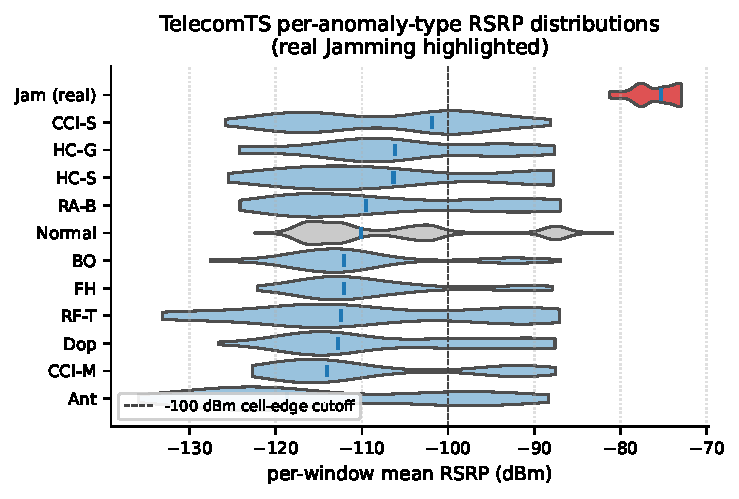
\includegraphics[width=.85\linewidth]{figures/E17_rsrp_per_type_distribution.pdf}}
  \caption{Per-anomaly-type RSRP distributions on TelecomTS.}
  \label{fig:e17_rsrp}
\end{figure}

\begin{figure}[t]
  \centering
  \scalebox{0.87}{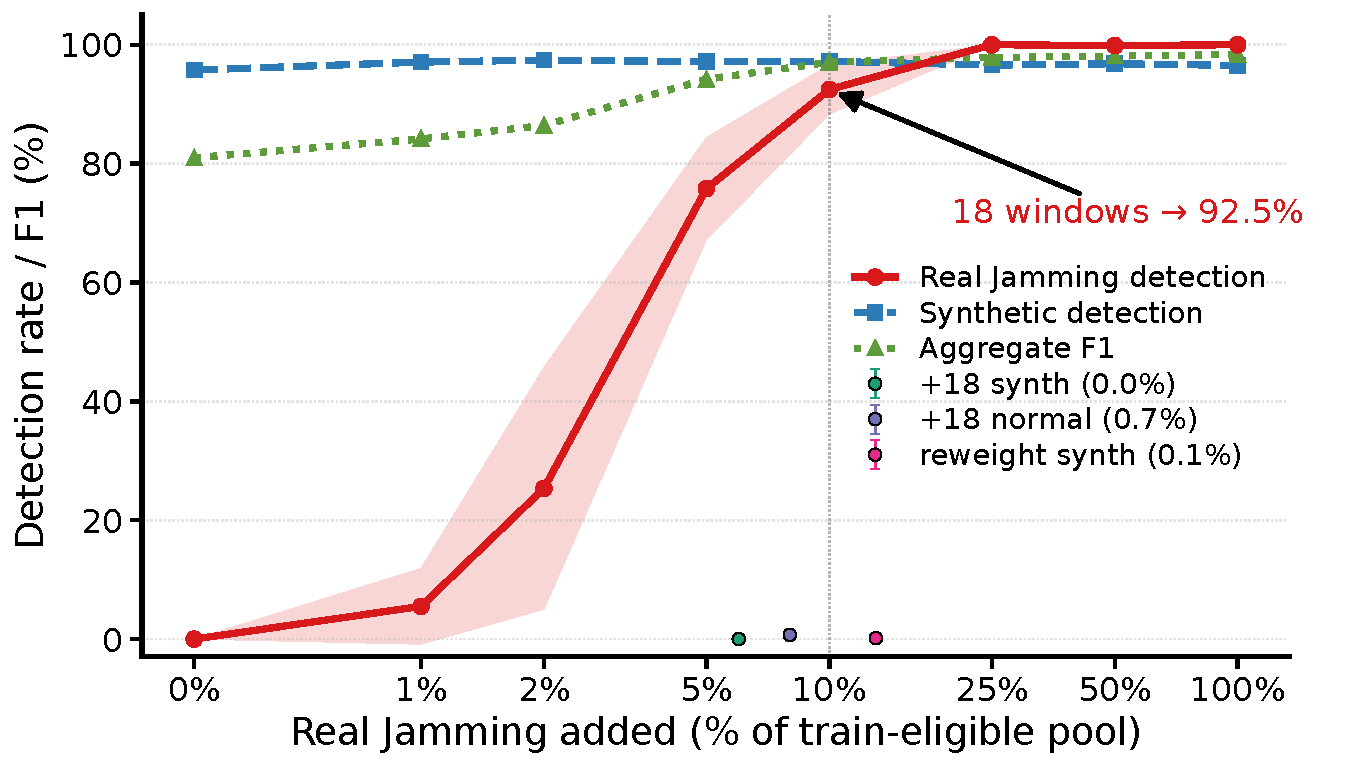
\includegraphics[width=.85\linewidth]{figures/E4_paper_optionA_with_controls.pdf}}
  \caption{Controlled-real calibration sweep on TelecomTS.}
  \label{fig:calibration}
\end{figure}

\subsection{Calibration Budget Estimation}
\label{sec:gap-repair}

We further estimate a \emph{per-corpus calibration budget}: the amount of controlled-real data required to recover reliable transfer for a given benchmark. This budget is not universal; it depends on the benchmark, fault origin, and operating-regime coverage. We therefore report it as an audit output rather than as a fixed recommendation. Let $f\in[0,1]$ denote the fraction of the train-eligible controlled-real pool added to synthetic-only training. On TelecomTS, the train-eligible pool contains 185 controlled-real Jamming windows, so $f=0.10$ corresponds to 18 windows. We sweep
\[
f\in\{0,0.01,0.02,0.05,0.10,0.25,0.50,1.00\}
\]
on the full-scale split while keeping the controlled-real test pool fixed across all sweeps. Figure~\ref{fig:calibration} visualizes the calibration curve together with matched-budget synthetic, normal, and reweighting controls, while Table~\ref{tab:m5_calibration_ci} reports the controlled-real recall statistics.

At $f=0$, controlled-real detection collapses to zero. By $f=0.10$, controlled-real recall rises to $0.92$ with worst-seed recall $0.86$, and by $f=0.25$ it saturates at $1.00$. Figure~\ref{fig:calibration} further shows that modest controlled-real calibration rapidly restores transfer, whereas matched-budget synthetic augmentation, additional Normal data, and synthetic reweighting do not produce comparable recovery. These results indicate a substantial operating-regime coverage gap that cannot be repaired by increasing synthetic data volume alone.

\paragraph{Why standard domain adaptation does not repair the gap.}
Standard covariate-shift correction methods are the natural alternative to controlled-real calibration when labels are scarce. We compare against importance weighting via logistic-regression density ratios~\citep{sugiyama2007covariate} and uLSIF-style least-squares importance fitting~\citep{kanamori2009ulsif}. As Table~\ref{tab:da_baseline} shows, neither method recovers controlled-real recall: IW-LR remains at $0.000$ recall and uLSIF-lite reaches only $0.009$, whereas modest controlled-real calibration restores recall to $0.93$.

The reason is structural rather than algorithmic. Importance weighting can only redistribute probability mass within the support already present in the synthetic-only training pool. The synthetic-only training pool does not contain windows occupying the controlled-real RSRP regime, so reweighting alone cannot recover the missing operating regime. The evidence indicates that the observed limitation stems from insufficient operating-regime coverage rather than from a mismatch in frequency distributions.

\begin{table}[t]
  \caption{Controlled-real calibration versus standard covariate-shift adaptation on TelecomTS.}
  \label{tab:da_baseline}
  \footnotesize
  \setlength{\tabcolsep}{3pt}
  \begin{tabular}{@{}lcccc@{}}
    \toprule
    Method & Real & Synth & $F_1$ & FPR \\
    \midrule
    (a) Synth-only baseline           & 0.001{\tiny$\pm$0.005} & 0.957 & 0.810 & 0.0006 \\
    (b) IW-LR (Sugiyama 2007)         & 0.000{\tiny$\pm$0.000} & 0.957 & 0.805 & 0.0009 \\
    (c) uLSIF-lite (Kanamori 2009)    & 0.009{\tiny$\pm$0.010} & 0.954 & 0.803 & 0.0011 \\
    (d) Real cal. $f\!=\!10\%$ (ours) & \textbf{0.93}{\tiny$\pm$0.07} & 0.970 & 0.969 & 0.0008 \\
    \bottomrule
  \end{tabular}
\end{table}

\begin{table}[t]
  \caption{Controlled-real calibration sweep on TelecomTS.}
  \label{tab:m5_calibration_ci}
  \footnotesize
  \setlength{\tabcolsep}{2.5pt}
  \begin{tabular}{@{}rrcccc@{}}
    \toprule
    $f$ & windows & mean & std & worst seed recall & 95\% CI \\
    \midrule
    0\%  &   0 & 0.00 & 0.00 & 0.00 & [0.00, 0.00] \\
    5\%  &   9 & 0.76 & 0.09 & 0.55 & [0.70, 0.81] \\
    10\% &  18 & 0.92 & 0.04 & 0.86 & [0.90, 0.95] \\
    25\% &  46 & 1.00 & 0.00 & 1.00 & [1.00, 1.00] \\
    100\%& 185 & 1.00 & 0.00 & 1.00 & [1.00, 1.00] \\
    \bottomrule
  \end{tabular}
\end{table}

\subsection{Cross-Corpus Replication}
\label{sec:cross-corpus}

\paragraph{Leave-one-anomaly-out (TelecomTS)}
The proposed audit systematically re-evaluates the synthetic-only protocol by iteratively holding out each anomaly type (Fig.~\ref{fig:e9b}a). Most held-out anomaly types remain recoverable because they share KPI neighborhoods with anomalies seen during training. The only major failure is the controlled-real Jamming type, whose recall collapses while recall on the remaining anomaly types remains high. The transfer failure is therefore not a generic property of held-out anomalies, but is specific to the controlled-real origin. Figure~\ref{fig:e9b}b further shows that controlled-real calibration selectively repairs the collapsed Jamming type while producing little change for already-generalizing anomaly families. The calibration procedure therefore acts on missing operating-regime coverage rather than uniformly boosting all anomaly types.

\paragraph{SpotLight Open RAN}
The presented audit reproduces both the distributional and transfer gaps when applied to the independent SpotLight corpus. Controlled-real and synthetic anomalies remain sharply separated in KPI space, but the dominant separating signals differ from TelecomTS: the primary separator is the layer-2 RLC-timer family rather than RSRP. The key finding therefore generalizes across two independent Open RAN testbeds even though the dominant KPI family responsible for the separation changes.

Under synthetic-only training, strong performance on synthetic anomalies is preserved while controlled-real \textsc{Radio} recall collapses across both tabular and raw-window detector families (Table~\ref{tab:s3_spotlight_transfer}). Controlled-real calibration again repairs the gap, although SpotLight requires a larger calibration budget than TelecomTS. The same calibration procedure therefore generalizes across corpora and detector families even though the absolute calibration budget remains corpus-specific.

\begin{figure}[t]
  \centering
  \scalebox{0.85}{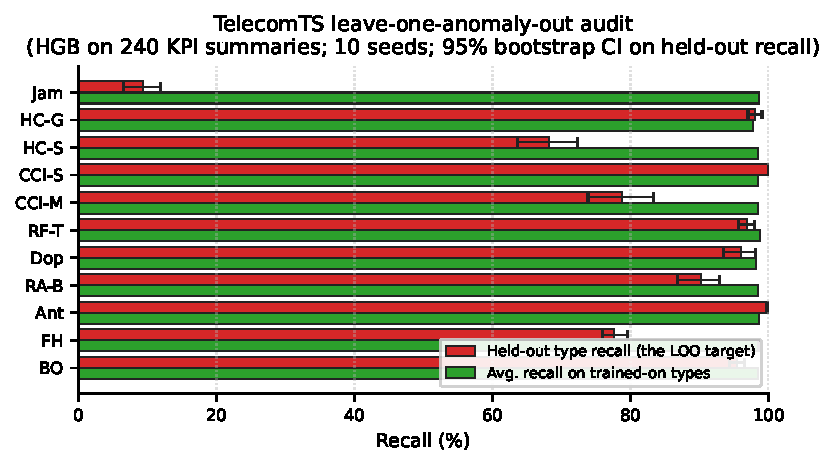
\includegraphics[width=\linewidth]{figures/E9b_leave_one_out_recall.pdf}}\\[-0.2em]
  {\footnotesize (a) leave-one-anomaly-out recall (10 seeds, 95\% bootstrap CI)}\\[0.5em]
  \scalebox{0.85}{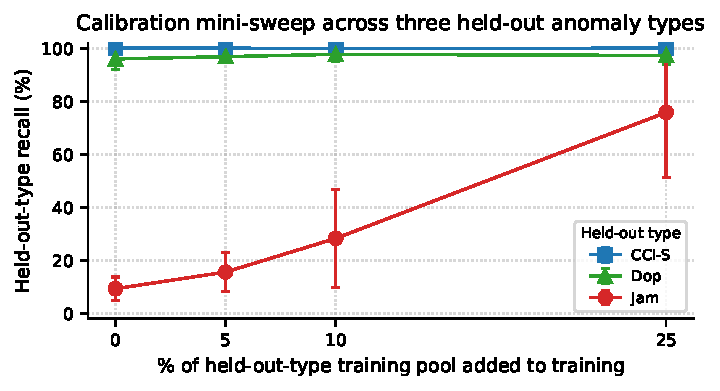
\includegraphics[width=\linewidth]{figures/E9b_calibration_minisweep.pdf}}\\[-0.2em]
  {\footnotesize (b) calibration mini-sweep on three held-out types}
  \caption{Leave-one-anomaly-out analysis on TelecomTS.}
  \label{fig:e9b}
\end{figure}

\begin{table}[t]
  \caption{Controlled-real calibration sweep on SpotLight.}
  \label{tab:s2_spotlight_cal}
  \footnotesize
  \setlength{\tabcolsep}{2pt}
  \begin{tabular}{@{}rrcccc@{}}
    \toprule
    $f$ & windows & \textsc{Radio} recall (95\% CI) & \textsc{Radio} miss \% & non-\textsc{R} recall & Normal FPR \\
    \midrule
    0\%   &   0 & 0.08 [0.01, 0.16] & 92\% [84\%, 99\%] & 0.97 & 0.03 \\
    10\%  &  21 & 0.67 [0.64, 0.70] & 33\% [30\%, 36\%] & 0.97 & 0.04 \\
    25\%  &  52 & 0.83 [0.79, 0.88] & 17\% [12\%, 21\%] & 0.99 & 0.06 \\
    50\%  & 103 & 0.87 [0.83, 0.91] & 13\% [9\%, 17\%]  & 0.96 & 0.06 \\
    100\% & 206 & 0.95 [0.94, 0.96] & 5\%  [4\%, 6\%]   & 0.98 & 0.08 \\
    \bottomrule
  \end{tabular}
\end{table}

\begin{table*}[t]
  \caption{Detector robustness of the real--synthetic transfer failure on SpotLight under synthetic-only and calibration results. Real denotes controlled-real \textsc{Radio} anomaly, and Synth denotes synthetic \textsc{Pdcp}/\textsc{Mac}/\textsc{Network} anomaly.}
  \label{tab:s3_spotlight_transfer}
  \footnotesize
  \setlength{\tabcolsep}{2pt}
  \begin{tabular*}{\textwidth}{@{\extracolsep{\fill}}lcccccccccccc@{}}
    \toprule
    Detector & \multicolumn{4}{c}{Synth-only ($f\!=\!0$)} & \multicolumn{4}{c}{Calibrated ($f\!=\!10\%$)} & \multicolumn{4}{c}{Calibrated ($f\!=\!25\%$)} \\
    \cmidrule(lr){2-5}\cmidrule(lr){6-9}\cmidrule(lr){10-13}
      & F1 & AUC & Synth & Real & F1 & AUC & Synth & Real & F1 & AUC & Synth & Real \\
    \midrule
    \multicolumn{13}{l}{Tabular detectors on per-channel KPI summaries} \\
    HGB            & 0.78{\tiny$\pm$0.03} & 0.94{\tiny$\pm$0.01} & 97{\tiny$\pm$3}\%  &\makebox[1.1pt][r]{\scriptsize$\rightarrow$\hspace{1.2pt}} 8{\tiny$\pm$12}\%  & 0.91{\tiny$\pm$0.01} & 0.98{\tiny$\pm$0.00} & 97{\tiny$\pm$2}\%  & 67{\tiny$\pm$5}\%  & 0.94{\tiny$\pm$0.01} & 0.99{\tiny$\pm$0.00} & 99{\tiny$\pm$1}\%  & 83{\tiny$\pm$7}\% \\
    RF             & 0.75{\tiny$\pm$0.02} & 0.92{\tiny$\pm$0.01} & 95{\tiny$\pm$4}\%  & \makebox[1pt][r]{\scriptsize$\rightarrow$\hspace{1pt}}  0{\tiny$\pm$0}\%   & 0.86{\tiny$\pm$0.06} & 0.97{\tiny$\pm$0.00} & 97{\tiny$\pm$4}\%  & 45{\tiny$\pm$24}\% & 0.91{\tiny$\pm$0.02} & 0.98{\tiny$\pm$0.00} & 98{\tiny$\pm$3}\%  & 77{\tiny$\pm$15}\% \\
    XGB            & 0.77{\tiny$\pm$0.01} & 0.92{\tiny$\pm$0.01} & 97{\tiny$\pm$2}\%  & \makebox[1.1pt][r]{\scriptsize$\rightarrow$\hspace{1.2pt}} 2{\tiny$\pm$2}\%   & 0.90{\tiny$\pm$0.02} & 0.98{\tiny$\pm$0.00} & 97{\tiny$\pm$3}\%  & 64{\tiny$\pm$12}\% & 0.92{\tiny$\pm$0.01} & 0.99{\tiny$\pm$0.00} & 98{\tiny$\pm$2}\%  & 80{\tiny$\pm$9}\% \\
    \midrule
    \multicolumn{13}{l}{Modern supervised detectors on raw $64\times452$ KPI windows} \\
    Toto (frozen)  & 0.80{\tiny$\pm$0.02} & 0.89{\tiny$\pm$0.00} & 90{\tiny$\pm$4}\% & 51{\tiny$\pm$10}\% & 0.81{\tiny$\pm$0.02} & 0.90{\tiny$\pm$0.01} & 91{\tiny$\pm$5}\% & 66{\tiny$\pm$12}\% & 0.84{\tiny$\pm$0.01} & 0.91{\tiny$\pm$0.01} & 92{\tiny$\pm$2}\% & 74{\tiny$\pm$8}\% \\
    TimesNet (e2e) & 0.73{\tiny$\pm$0.04} & 0.85{\tiny$\pm$0.01} & 94{\tiny$\pm$8}\% &\makebox[1.1pt][r]{\scriptsize$\rightarrow$\hspace{1.2pt}}  1{\tiny$\pm$2}\%   & 0.84{\tiny$\pm$0.05} & 0.94{\tiny$\pm$0.01} & 99{\tiny$\pm$2}\% & 43{\tiny$\pm$25}\% & 0.90{\tiny$\pm$0.04} & 0.95{\tiny$\pm$0.01} & 98{\tiny$\pm$4}\% & 81{\tiny$\pm$14}\% \\
    \bottomrule
  \end{tabular*}
\end{table*}

\paragraph{Why does SpotLight require more calibration than TelecomTS}
This follows directly from the two-component gap structure identified 
in Table~\ref{tab:e16_ablation}: when the coverage gap is concentrated 
on a single KPI axis (RSRP in TelecomTS's 16-channel space), a small 
calibration budget suffices; when it is distributed across many 
features (as in SpotLight's 452-channel RLC-timer family), each 
calibration window carries less information about the dominant regime 
shift, and more controlled-real coverage is required before transfer 
stabilizes.

%% ====================================================================
\section{Applied Deployment Evidence}
\label{sec:applied}
%% ====================================================================

The primary contribution of this work is not a new anomaly detector, but a deployment-oriented benchmark-auditing gate for determining whether benchmark evidence is sufficiently reliable to support model promotion. Our proposed framework therefore provides three complementary forms of applied evidence to support practical evaluation and deployment readiness: \emph{(i)} a publicly available reproducibility pipeline within our proposed framework that reconstructs the principal audit results reported in this study, \emph{(ii)} cross-corpus validation within our proposed framework across two independent public 5G/Open RAN testbeds, demonstrating consistent behavior under heterogeneous deployment conditions, and \emph{(iii)} pre-production shadow-mode integration inside Nokia's anomaly-detection pipeline. Across these settings, origin-aware auditing changes the deployment decision: models that seem acceptable under aggregate $F_1$ are downgraded to rejection or shadow-mode deployment once anomaly-origin–aware auditing is applied.

\begin{table}[t]
  \caption{Applied evidence and measured utility of the released audit workflow within the proposed framework.}
  \label{tab:release}
  \footnotesize
  \setlength{\tabcolsep}{3pt}
  \begin{tabular}{@{}lp{0.62\linewidth}@{}}
    \toprule
    \textbf{Dimension} & \textbf{Evidence} \\
    \midrule
    Public release &
    MIT-licensed repository with source codes, cached embeddings, environment file, and shared audit module. \\
    Reproducibility &
    Core public audit regenerates the TelecomTS/SpotLight tables and figures in ${\sim}30$ minutes without GPU. \\
    Benchmarks &
    TelecomTS, SpotLight, and Nokia internal timing-flow benchmark. \\
    Decision impact &
    Aggregate-$F_1$ detector accepted under standard reporting but rejected or held in shadow mode under origin-aware reporting. \\
    Calibration utility &
    TelecomTS: 18 controlled-real windows restore recall to 0.92; SpotLight: 52 windows restore \textsc{Radio} recall to 0.83. \\
    Nokia integration &
    Pre-production audit module with programmatic interfaces, CI gating, and shadow-mode evaluation. \\
    Runtime overhead &
    $<1\,\mu$s per inference in the measured Nokia service path; median CSV audit time 0.15\,s. \\
    \bottomrule
  \end{tabular}
\end{table}

\subsection{Operator-facing workflow}
The audit is designed for an MLOps engineer or benchmark owner before detector promotion. The workflow is: label anomaly windows by origin; report recall by origin rather than only aggregate $F_1$; test controlled-real versus synthetic anomaly distributions with C2ST/MMD; run train-on-synthetic/test-on-controlled-real evaluation at the natural anomaly rate; and estimate the smallest controlled-real calibration budget that restores origin-conditioned recall. The released toolkit emits an operator-facing verdict that either permits standard model selection, requires controlled-real calibration, or blocks benchmark-based certification until controlled-real or operator-confirmed fault evidence is available.

\subsection{Nokia pre-production integration}
\label{sec:nokia-deployment}
We integrated our proposed auditing framework into Nokia’s \emph{Agentic Anomaly Detection} platform as a pre-production audit module supporting programmatic APIs, automated CI gating, and shadow-mode evaluation workflows. The integration is not part of production serving; instead, it gates benchmark certification and detector-promotion decisions before models are allowed to move beyond shadow evaluation.

\paragraph{Measured Nokia decision impact.}
We evaluated the audit gate on a Nokia internal timing-flow benchmark containing $3{,}958$ windows and $203$ KPI features. Under aggregate reporting, an HGB detector would pass the existing validation gate: AUROC $\approx0.99$ at the natural rate with $F_1\approx0.77$, and AUROC $\approx0.96$ at a balanced rate with $F_1\approx0.92$. Under origin-aware reporting, the same benchmark is flagged as containing only synthetic anomalies: every anomalous window is synthetic, so the benchmark provides no controlled-real or operator-confirmed fault evidence. The promotion decision therefore changes from ``accept'' to ``hold in shadow mode pending real-origin evidence.'' A data-sanity diagnostic on the same benchmark also shows strong Normal--synthetic separability (C2ST accuracy $0.992$, AUROC $0.996$, MMD $78.1\times$ the permutation-null mean, $p=0.002$), confirming that the audit surfaces benchmark structure before deployment.

\paragraph{Shadow-mode usage and overhead.}
The audit has run as a CI gate over every Nokia timing-flow CSV in the current in-house workspace: four CSVs, $15{,}376$ windows, and $4.27$ hours of timing-flow data. It held all three candidate detectors in shadow mode and correctly marked the baseline-traffic CSV as \texttt{no\_anomalies\_present}. The operator-facing output is a single JSON verdict consumed by the existing CI/CD pipeline. The measured cost is small enough for every benchmark refresh: median wall-clock time is $0.15$\,s per CSV, p95 is $0.21$\,s, and service-path overhead is below $1\,\mu$s per inference on single-thread CPU.

\paragraph{Deployment lesson.}
The applied lesson is that high aggregate benchmark scores are not sufficient certification evidence when anomaly origins are incomplete or distributionally separated. In the Nokia case, the audit does not claim the candidate detector is bad; it shows that the benchmark is insufficient to certify controlled-real transfer. This distinction is important operationally: the correct action is not to tune another model on the same synthetic benchmark, but to collect controlled-real calibration evidence, obtain operator-confirmed incidents, or keep the detector in shadow mode until such evidence exists.

\subsection{Released artifact and reproducibility}
The audit toolkit is publicly released under the MIT License.\footnote{Cached embeddings and reproduction source codes: \url{https://github.com/ChimanSalavati/telecomts-real-synthetic-gap}.}
The release includes reproduction source codes, cached embeddings, environment configuration files, and a shared Python module supporting split auditing, origin-conditioned evaluation, C2ST/MMD diagnostics, calibration sweeps, and cross-corpus replication. The core auditing pipeline reproduces the main public-corpus tables and figures in approximately 30 minutes without requiring a discrete GPU. To support robust and resumable execution, we also provide checkpointed per-seed outputs that allow interrupted runs to resume without recomputing completed seeds. Collectively, these artifacts make the publicly released portion of the evidence independently verifiable without reliance on Nokia-internal access.
%% ====================================================================
\section{Conclusion and Limitations}
\label{sec:conclusion-limits}
%% ====================================================================

Reliable deployment of telecom anomaly detectors depends not only on detector architecture, but also on whether benchmark anomalies represent the fault regimes operators need to detect. We operationalized this idea as \emph{origin-aware benchmark auditing}: a workflow that reports performance by anomaly origin, diagnoses whether synthetic anomalies cover controlled-real KPI regimes, and estimates the controlled-real calibration needed before a benchmark can support model promotion.

Across two public 5G/Open RAN testbeds and a pre-production Nokia anomaly-detection pipeline, the audit exposes a failure mode hidden by aggregate metrics. Synthetic-only training can preserve strong performance on synthetic anomalies while missing controlled-real faults. The evidence indicates that this failure arises from insufficient operating-regime coverage rather than detector choice, a single leaked feature, or standard covariate-shift frequency mismatch. In that setting, additional synthetic or normal data is not a substitute for controlled-real calibration.

This work has several limitations. The audit focuses on KPI-distribution evidence and does not incorporate multimodal observability signals such as alarms, tickets, or textual reports. Calibration requirements are corpus-specific rather than universal, and released TelecomTS metadata does not support fully group-aware session splits. In addition, large-scale raw-window transformer modeling on Open RAN telemetry remains computationally demanding and is better treated as an artifact-level extension than as the central contribution of this work.

%% ====================================================================
\section*{GenAI Usage Disclosure}
In this work, generative AI tools were used to assist with grammar checking, sentence clarification, and submission-readiness review of the manuscript.


\bibliographystyle{ACM-Reference-Format}
\bibliography{references}

\end{document}
